\chapter{Accurate Prediction of the Refractive Index of Organic Polymers}

We present an efficient computational protocol for the accurate prediction of RI values in polymers to facilitate \insilico\ studies that can guide the discovery and design of next-generation high-RI materials. Our protocol is based on the Lorentz-Lorenz equation and is parametrized by the polarizability and number density values of a given candidate compound. In the proposed scheme, we compute the former using \firstprinciples\  electronic structure theory and the latter using an approximation based on van der Waals volumes. The critical parameter in the number density approximation is the packing fraction of the bulk polymer, for which we have devised a machine learning model. We demonstrate the performance of the proposed RI protocol by testing its predictions against the experimentally known RI values of 112 optical polymers. Our approach to combine \firstprinciples\  and data modeling emerges as both a successful and highly economical path to determining the RI values for a wide range of organic polymers.

We thank Prof. Chong Cheng for helpful discussions on the scope of high RI polymers and synthetic feasibility of new polymers. The results of this study were published in ‘M. A. F. Afzal, C. Cheng, J. Hachmann, J. Chem. Phys. 128 (2018), 144101’ \cite{Afzal2018a}, and this chapter is based on our exposition in this paper. 

\section{Introduction}
% Provide the general context: list different kinds of organic materials, state wide-ranging importance, discuss unique or desirable properties compared to conventional materials [keep this relatively short - maybe 2-3 sentences or so]
Organic small molecules, oligomers, and polymers are emerging materials and of significant interest for numerous fields of application due to their unique or otherwise desirable properties \cite{Higashihara2015}. Unlike most conventional inorganic materials, they are generally flexible, light-weight, mechanically stable on impact, easy to process, and inexpensive to produce \cite{Lu2005,Zimmermann1993}. Perhaps most importantly, their properties can be tailored towards specific demands by controlling their molecular structure \cite{Liu2009}.
% Narrow down the context: Applications of organic polymers with a focus in optics and optoelectronics; give a number of examples [keep this relatively short - maybe 2-3 sentences or so]
A particular area of interest is the application of organic materials in optic and optoelectronic devices \cite{Lei2014}, such as (image) sensors \cite{Angione2011, Voigt2011}, displays \cite{Ummartyotin2012}, and light sources (including organic light-emitting diodes) \cite{Xiang2017}, in which they can be introduced \insitu\  as microlenses \cite{Nishiyama2009}, waveguides \cite{Kokubun1993}, microresonators \cite{Wei2016}, interferometers \cite{Rodriguez2001}, anti-reflective coatings \cite{Singaravalu2013}, optical adhesives \cite{Kim2013}, and substrates  \cite{Kim2015}. Some of the optical properties that are relevant for these applications are the refractive index (RI), Abbe number, birefringence, absorption spectrum, and color \cite{Sun2008}.   

% Zoom in on refractive index as an important optical property. Mention the importance of high refractive index (>1.7) materials 
The RI value dictates the shape and size of many optical components, in particular those with lens function. Most of the aforementioned applications require materials with large RI values (\ie  larger than 1.7), and there are several applications that require very large ones (\ie  larger than 1.8) \cite{Jintoku2014}. Unfortunately, the vast majority of organic polymers only offer RI values ranging from 1.3 to 1.5 \cite{Liu2009} (compared to inorganic materials, which can feature values up to $\sim$4). 
% Now that we have established that this is an interesting and relevant field, introduce various strategies to increase the RI value in organic materials, and why we are not there yet
The development of high-RI polymers has thus gained attention, and several approaches have been proposed to overcome the RI-value limitations of typical organic polymers. They include the notion to incorporate highly polarizable moieties, such as rigid aromatic fragments \cite{Seto2010}, heteroatoms \cite{Griebel2014,Tojo2013}, or organometallics \cite{Ho2009}, into the polymer scaffold. Another strategy that has been pursued is to reinforce the polymer matrix with metal alkoxides (\eg  \ce{TiO2}, \ce{Fe3O4}) \cite{Liu2013,Parke2013} or other high-RI molecules (\eg  \ce{ZnS}, diamondoids) \cite{Zhang2014,Robello2013}. While these approaches have resulted in a few systems with RI values between 1.6 and 1.8, most of them are of limited utility for practical applications due to a variety of materials, processability, or preparation issues \cite{Liu2009}. Increasing the RI values of organic polymers beyond 1.8 has remained a completely elusive task and continues to be an important challenge in synthetic chemistry \cite{Griebel2014}. 

% Introduce the problem setting that this paper tries to address, i.e., explain the limitations, shortcomings to the traditional, experimental discovery process for high-RI polymers
The traditional, experimentally focused discovery process for new materials is very time-, labor-, and resource-intensive, which limits the number and diversity of candidate compounds that can be explored. Progress thus tends to be slow and incremental, in particular for advanced materials systems, which require more and more intricate property profiles.
% Make case for in silico research in order to overcome shortcomings by supporting, guiding experimentalists, mention MGI; don't bash experiment but show how joint ventures are the path to progress [you can potentially reuse some of the text from my CAREER proposal here; don't go into technical detail but stay with a big picture level]
However, chemical and materials research has been undergoing a significant transformation in recent years that can alleviate many of these shortcomings: After decades of continuous advances in methods, algorithms, and computer hardware, the fields of modeling and simulation have reached a tipping point, and they are finally at a stage where they can make accurate predictions for systems that are both realistic and relevant. Progress is now increasingly driven by computational studies, which have become crucial assets in the pursuit of next-generation materials and chemistry. By making guiding predictions, they can significantly boost the efficiency of research endeavors, and uncover promising targets for investigations in the laboratory (see, \eg  Ref.\ \cite{cep01,Sokolov2011,Hachmann2011,Olivares-Amaya2011,Amador-Bedolla2013,Hachmann2014,Pyzer-Knapp2015,Lopez2016}). The White House Materials Genome Initiative \cite{NationalMaterials2011} underscores the value of integrated joint ventures between experimentalists and theoreticians in tackling complex discovery and design challenges and delivering revolutionary new materials.
%\textcolor{red}{
A prominent example in the context of optical materials is the work by Ramprasad and co-workers \cite{Huan2016,Sharma2014,Mannodi-Kanakkithodi2016}, which we will use as a reference point.
% }

% Point out the prerequisite for this approach: having a suitable computational protocol for predicting the RI of polymers, i.e., developing this paper is about developing such a protocol
A prerequisite for the computationally-driven development of new materials is access to suitable (\ie  accurate and efficient) computational protocols for the target property within a compound space of interest. This paper presents such a protocol for the prediction of RI values of organic polymers. One of the distinctive feature of this protocol compared to prior work by others \cite{Huan2016,Sharma2014,Redmond2011,Park2011} is that it fuses \firstprinciples\  and data modeling. 

% outline of paper
In Sec.\ \ref{sec:methods}, we introduce the physical foundations of the proposed protocol (Sec.\ \ref{subsec:lorentzlorenz}), 
motivate a number of assumptions and approximations that are used (Sec.\ \ref{subsec:polarizability} and \ref{subsec:numberdensity}), and discuss the details of the employed computational approach (Sec.\ \ref{subsec:compdetails}). In Sec.\ \ref{sec:results_discussion}, we present and discuss results for the different components that comprise the protocol (Sec.\ \ref{subsec:polarizability_results}, \ref{subsec:numberdensity_results}, and \ref{subsec:packingfractions_results}) as well as the overall protocol itself (Sec.\ \ref{subsec:RI_results}). In each case, we evaluate the predictive performance of our model by comparing its results with data from a validation set of experimentally known compounds. Sec.\ \ref{subsec:interplay_results} provides a discussion of the interplay between the physical parameters of our model. Our findings are summarized in Sec.\ \ref{sec:conclusions}.



\section{Background and Methods}
\label{sec:methods}
\subsection{Lorentz-Lorenz Equation}
\label{subsec:lorentzlorenz}
% Connection of the refractive index with the polarizability and number density via the Lorentz-Lorenz equation [logic/argument from presentation slides]
The RI value ($n_r$) is defined as the ratio between the speed of light in vacuum ($c_0$) and in a given material ($c$). For non-magnetic materials, the RI is thus the square root of its relative permittivity 
% \textcolor{red}{
or dielectric constant 
% }
($\epsilon_r$), \ie 
$$n_r=\dfrac{c_0}{c} = \sqrt{\epsilon_r}.$$
The permittivity is a function of the polarizability ($\alpha$) and using the Lorentz local field approximation, it can be written as
$${\epsilon{}}_r=\frac{1+2\alpha{}N/{3\epsilon{}}_0}{1-\alpha{}N/{3\epsilon{}}_0},$$
where $N$ is the number density, \ie   the number of molecules per volume. It follows that the RI is
$$n_r=\sqrt{\frac{1+2\alpha{}N/{3\epsilon{}}_0}{1-\alpha{}N/{3\epsilon{}}_0}},$$
which is a version of the Lorentz-Lorenz equation (equivalent to the Clausius-Mossotti relation). It follows, that the Lorentz-Lorenz equation connects the macroscopic RI value of a bulk material to the electronic polarizability $\alpha$ and number density $N$ of its molecular constituents.
% Give a brief summary of the physical basis of the RI protocol 
The Lorentz-Lorenz equation thus offers a route to calculating the RI value of a material \via\ $\alpha$ and $N$, and we use it as the physical basis for the proposed computational protocol (for a detailed discussion of this approach see App.
\ref{appendix:A}).  


\subsection{\textit{First-Principles} Molecular Polarizability Calculations}
\label{subsec:polarizability}
% Introduce general notion of molecular polarizability calculations, issue of dispersion
The polarizability $\alpha$ of a compound can be obtained from quantum chemical linear response calculations. An array of electronic structure methods has been used to determine the polarizability values of various materials \cite{Ando2006,Rocquefelte2004,Jensen1983,Rabah2003,Amrani2006,Reshak2014,Azam2013}, including organic polymers \cite{Ksianzou2006,Zeinalipour-Yazdi2008,Yu2007}. Polarizability is generally a frequency-dependent (\ie  dynamic) property as shown in Fig.\ \ref{fig:pol_wl}. Frequency-dependent polarizability is relatively hard to compute, as it formally involves solving the time-dependent Schr\"odinger equation and/or scanning through the range of relevant frequencies \cite{Rao2013}. Consequently, only relatively few studies consider the polarizability dispersion in organic polymers \cite{Rowan2011,Lenz2011}. 

\begin{figure}[htbp] 
	\centering
	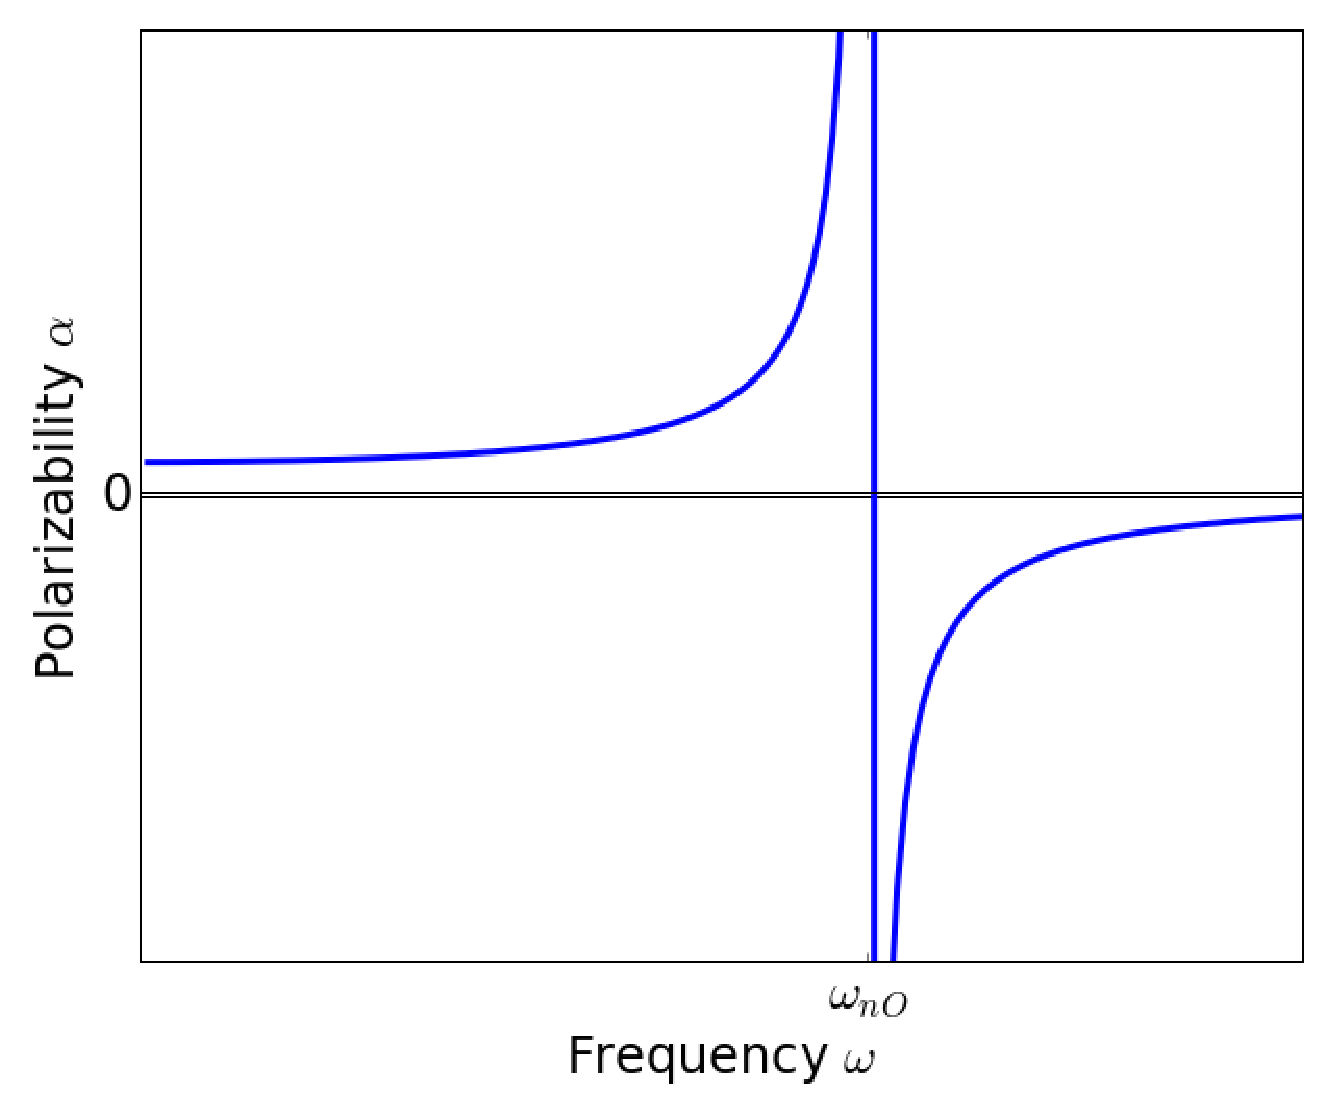
\includegraphics[width=0.6\textwidth]{Chapter-2/Figures/RI_vs_freq.eps}
	\caption{Dispersion characteristic of the polarizability: Excited states are marked by singularities, and in the frequency range below, the polarizability converges asymptotically towards the constant static polarizability value.} 
	\label{fig:pol_wl} 
\end{figure}  

% go to RI, argue why we get away with using frequency independent solution/static polarizability
From the frequency dependence of the polarizability follows that the RI is also a frequency-dependent property. However, the variation of both polarizability and RI in the visible frequency region is in fact often relatively small \cite{Robello2013}, as long as low-lying excited states are absent. Since the latter would render a material unsuitable for optical applications anyways, we generally do not consider materials that exhibit them. Large variations can be observed in the ultraviolet region where resonances with the excited state manifold become a dominant feature, but since stability considerations prohibit organic polymers to be used for high-energy applications, this is also not a relevant concern. Below the frequency range of the excited states, the polarizability and RI value taper off monotonically (cf.\ Fig.\ \ref{fig:pol_wl}). In most cases, they become essentially constant throughout the visible and infrared range and converge to an asymptotic value \cite{Robello2013}. The asymptotic RI corresponds to the value that can be obtained from the static polarizability. The latter can be computed much more easily than the frequency-dependent value. It only requires a single linear response calculation without explicit time dependence, and is thus much less demanding in terms of computing time and numerical stability. We can conclude that the RI values obtained from static polarizability calculations form a close lower bound for the frequency-dependent values in the relevant spectral range. This approach has been used in the past and has given very good agreement with experimental results \cite{Azim-Araghi2012,Ksianzou2006,Lee2011,Park2011,Zeinalipour-Yazdi2008}.

% move on to challenge of calculating polymer values
Another challenge is to perform the polarizability calculations for quasi-infinite polymers. 
% outline issues: PBC tricky and not realistic, explicit polymer calcs too expensive
Realistic systems are amorphous and may thus not be well represented by periodic boundary condition calculations, while non-periodic calculations on long-chain oligomer models are generally cost-prohibitive. 
% solution via extrapolation scheme: make use of short correlation length, extensivity of optical properties
However, for systems with a relatively short correlation length (\eg  due to finite conjugation and delocalization of the $\pi$-electron backbone), we can expect an early onset of extensivity in the optical properties. We can exploit this behavior through an extrapolation scheme. 
% explain extrapolation scheme, i.e., talk about polymer values from molecular ones: polymer polarizability values can be obtained from small chain oligomers results using extrapolation scheme  
In this scheme, we perform a series of relatively simple monomer and small oligomer calculations until we observe a linear trend in the polarizability results, based on which we can project 
%from the molecular results 
to the polymer limit.

% talk about DFT, cost vs accuracy -> basis set dependence, scaling, prior benchmark study
The molecular polarizability calculations in the proposed protocol utilize Kohn-–Sham density functional theory (DFT) for its advantageous trade-off of cost and accuracy \cite{Neese2009}. The former includes its low-order polynomial scaling with system size and its relatively modest basis set demands (compared to high-level wavefunction methods).
%; the latter has been shown in prior benchmark studies 
% discuss geometries and geometry optimization; justify 
Given the molecular-level disorder in amorphous polymers, we forgo the expensive \firstprinciples\  optimization of idealized geometries of our candidate compounds in favor of an inexpensive molecular mechanics approach. 
% mention that we check for low lying excited states by assessing HOMO-LUMO gap
A simple, yet efficient way to identify (and exclude) compounds with potentially low-lying excited states is to assess the gap between the highest occupied molecular orbital (HOMO) and the lowest unoccupied molecular orbital (LUMO). The HOMO--LUMO gap is a first approximation for the lowest excitation, and it is readily obtained in DFT at no additional cost.  



\subsection{Data Model for the Number Density}
\label{subsec:numberdensity}
% introduce MD as conventional approach to compute number density
The number density $N$ for amorphous polymers is typically computed using classical molecular dynamics simulations. 
% MD is a time consuming and complicated approach that does not scale well for the long-term goal of screening 
However, this approach is relatively cumbersome and computationally demanding.
% we try to avoid it and instead bypass it using the using an approximation based on the Van der Waals volume; mention that for this we need to know the vdW volume and packing fraction 
As an alternative, we pursue an approach based on the molecular volume (approximated by the van der Waals volume $V_{vdW}$), \ie 
$$N=\frac{K_p}{V_{vdW}},$$
where $K_p$ is the packing fraction in the bulk polymer, which has shown good agreement with experimental results in other work \cite{Liu2008a,Terui2004}. 
% mention that there are many different approximations for how to compute the former (list these), but that a comparison indicates that the differences are relatively small so that we utilize a more simplistic scheme 
There are a number of ways to compute the van der Waals volume, ranging from complicated electronic structure calculations with subsequent partitioning of the electron density to simplistic fragment methods \cite{Lu2012,Zhao2003}. A benchmark study that we will detail elsewhere has shown that the differences in results from different methods are generally small. For the present work, we thus adopt the latter, \ie  we calculate $V_{vdW}$ by adding tabulated atomic values \cite{Bondi1964} and subtracting off the overlap in the bonding region. 
% Discuss that packing fraction is given as a constant in the literature but that this is an average with large standard deviation which makes it useless
The average packing fraction $K_p$ for organic polymers is given in the literature as 0.68 \cite{askadski2003}, however, the actual values of different polymers show a significant spread and are known to range at least from 0.5 to 0.8. ($K_p$ is generally also a function of the degree of polymerization, but except for shorter oligomers, this only plays a minor role.)  
% Introduce machine learning approach for the prediction of the packing fraction. Mention on a basic level the choice of approach and motivation
As the average value of this critical parameter is thus essentially meaningless, we have devised a machine learning model to correlate the polymer structure with its packing fraction. Due to the relatively small volume of available training data, we chose a comparatively inflexible (but exceedingly fast) support vector regression (SVR) approach to avoid overfitting. 
% \textcolor{red} {
Modern support vector machines were introduced in 1992 for supervised classification problems and have been a popular machine learning technique since their inception \cite{Boser1992}. A version for regression analysis was added in 1996 \cite{drucker1997,smola2004}. Non-linear SVR prediction models are generated by projecting the training data into a high-dimensional kernel-induced feature space where they become linear regression problems subject to cost functions that penalize prediction errors.
% }


\subsection{Computational Details}
\label{subsec:compdetails}
The polarizability calculations of the proposed protocol use an all-electron, restricted DFT framework with the PBE0 hybrid functional \cite{Adamo1999} in combination with the triple-$\zeta$ quality def2-TZVP basis set by the Karlsruhe group \cite{Weigend2005}. We include Grimme's D3 correction \cite{Grimme2010} to account for dispersion interaction. The proof-of-principle study shown in the following section was carried out using the ORCA 3.0.2 quantum chemistry program package \cite{Neese2012} with default settings. We optimized the geometries of all monomers and oligomers using the universal force field (UFF) \cite{Rappe1992} as implemented in the OpenBabel software \cite{OBoyle2011}. We calculated the van der Waals volumes using Slonimskii's method detailed in Ref.\ \cite{Slonimskii1970}, for which we implemented a Python script.
% detail the ML algorithm and details of the parameters used. Subsequently, give details of the descriptors used for the ML model.
We generated the packing fraction model using SVR within a feature space of 43 constitutional descriptors on a training data set of 84 polymers with experimentally known $K_p$ values compiled from the literature. The available data was divided into 80\% training and 20\% test set for cross-validation. 
The data modeling was performed using \chemml\ \cite{Haghighatlari2017}, our program suite for machine learning and informatics in chemical and materials research. In this work, \chemml\ employed the scikit-learn 0.17 SVR library \cite{scikit-learn} and descriptors from Dragon 7 \cite{Taletesrl2011}.
% Mention ChemHTPS to perform RI calculation on 112 polymers [keep this short to 1-2 sentences and refer to future publications on the details; you don't want to muddy the two stories]. 
The proof-of-principle study involved about 450 individual calculations, which we performed using \chemhtps\ \cite{Afzal2018c}, our program suite for automated virtual high-throughput screening in chemical and materials research.  



\section{Results and Discussion}
\label{sec:results_discussion}
% Results of polarizability calculation of non-conjugated polymers polyethylene (PE) and polystyrene (PS) as example polymers, subsequently known polymers.  
We developed the proposed RI protocol on two common non-conjugated polymers -- polyethylene (PE) and polystyrene (PS) -- as prototype systems. Subsequently, we performed a study of 112 non-conjugated polymers for which experimental RI values are known in order to validate the predictive performance of the RI protocol as well as its individual components. 

\subsection{Polarizabilities}
\label{subsec:polarizability_results}
% Linear dependence and easy extrapolation scheme; point out that this is valid for non-conjugate polymers and that for conjugated ones this may not be the case, cite Dupuis paper
The PBE0/def2-TZVP-D3 polarizability results for PE and PS from monomer to heptamer are shown in Fig.\ \ref{fig:pol_lin}. The linear trend with respect to the number of monomer units $n$ (due to extensivity) is easily recognized. The correlation coefficient $R^2$ for the linear regression is $\gg0.99$. For all cases studied in this work, extensivity was observed for very short oligomer sequences, and we based our extrapolation scheme on the linear regression slope obtained from the monomer to tetramer results.


\begin{figure}[htbp] 
	\centering
	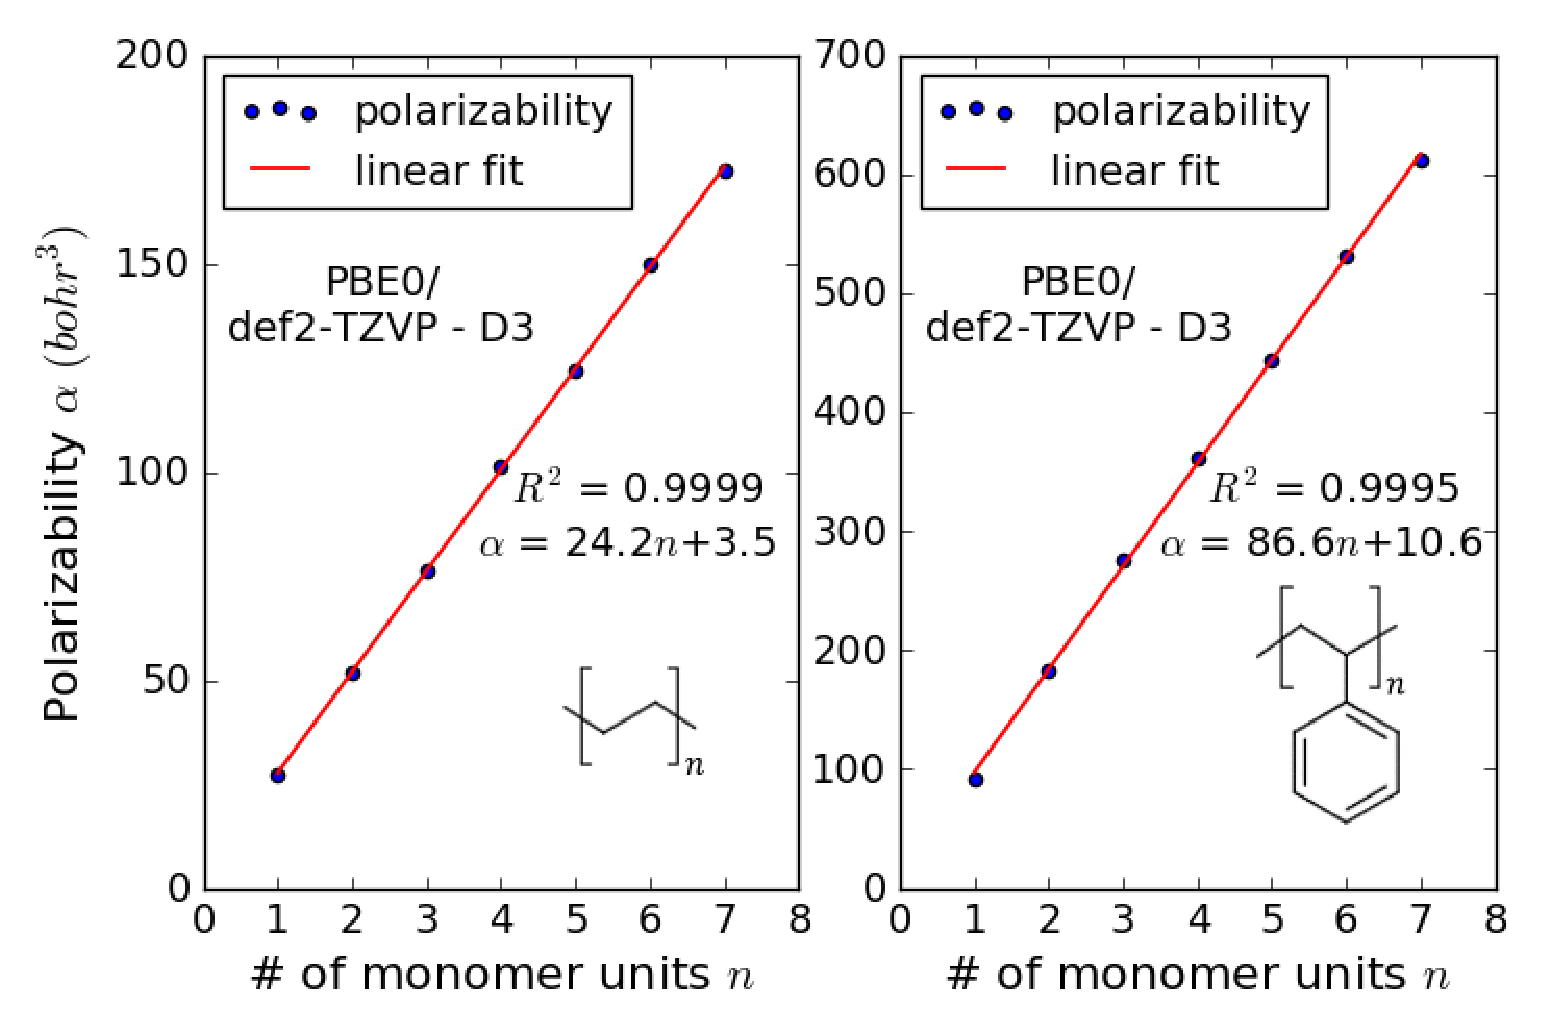
\includegraphics[width=0.75\textwidth]{Chapter-2/Figures/plot_pol.eps}
	\caption{Linear relationship between number of monomer units and polarizability for polyethylene (PE) and polystyrene (PS) as prototypes for non-conjugated polymers.} 
	\label{fig:pol_lin} 
\end{figure}  

Note that for conjugated polymers with longer correlation lengths, the onset of extensivity can occur at significantly longer chain length, \ie  values for a sequence of shorter oligomers will not show a linear trend \cite{Dupuis1988,Mosley1994}. 
% \textcolor{red} {
An example is given in Fig.\ \ref{fig:pol_non_lin}. 
% }
The extrapolation scheme can still be used in these cases, but it requires the calculation of longer oligomer sequences until a linear trend for extrapolation is found. 

\begin{figure}[htbp] 
	\centering
	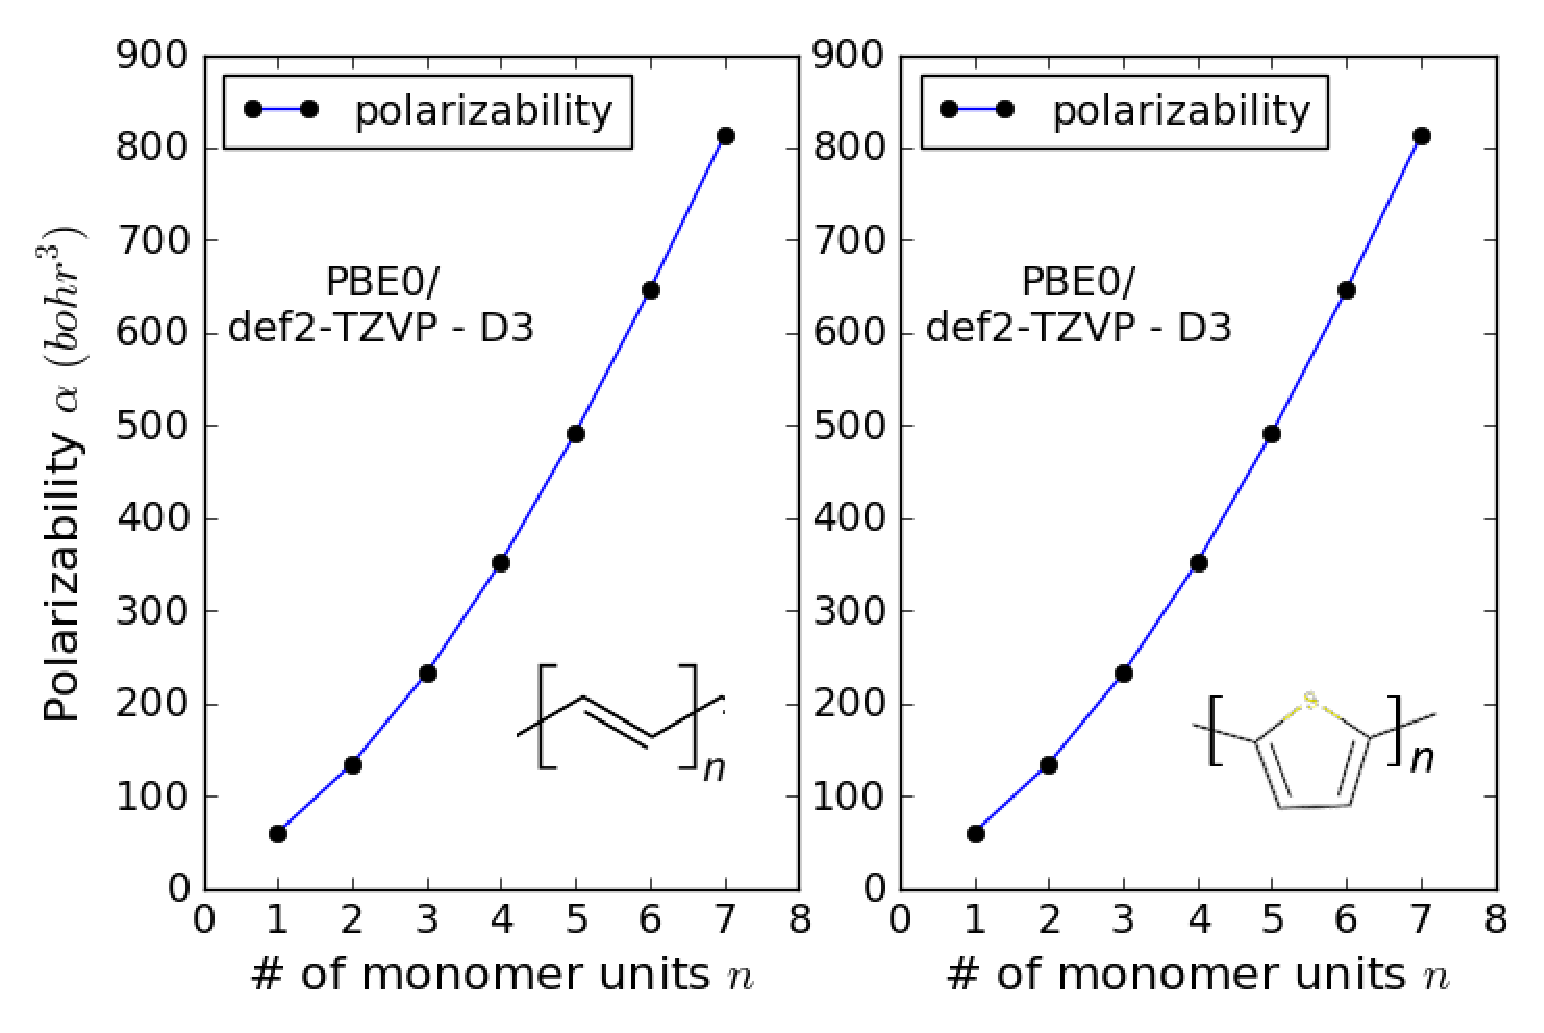
\includegraphics[width=0.75\textwidth]{Chapter-2/Figures/PA_PT_pol.eps}
	\caption{Non-linear relationship between number of monomer units and polarizability for polyacetylene and polythiophene as prototypes for conjugated polymers.} 
	\label{fig:pol_non_lin} 
\end{figure}  



\subsection{Number Densities and Densities}
\label{subsec:numberdensity_results} 
% Results of number density calculation of bulk polymers of PE and PS; this will be straight forward from vdW volume, as we already know the packing fraction of these polymers. 
Using Slonimskii's method we could readily compute the van der Waals volumes $V_{vdW}$ for the prototype systems PE and PS. Assuming the average packing fraction of $K_p = 0.68$, we obtain the number density values $N$ as a function of the number of monomer units $n$ shown in Fig.\ \ref{fig:nden_ex}.  
% Discuss the variation of number density with chain length using the same packing fraction for all oligomer length. 
The plots illustrate that $N$ decreases monotonically with increasing number of monomer units, and the inverse $1/N \propto V_{vdW}$ is evidently extensive. 


\begin{figure}[htbp] 
	\centering
	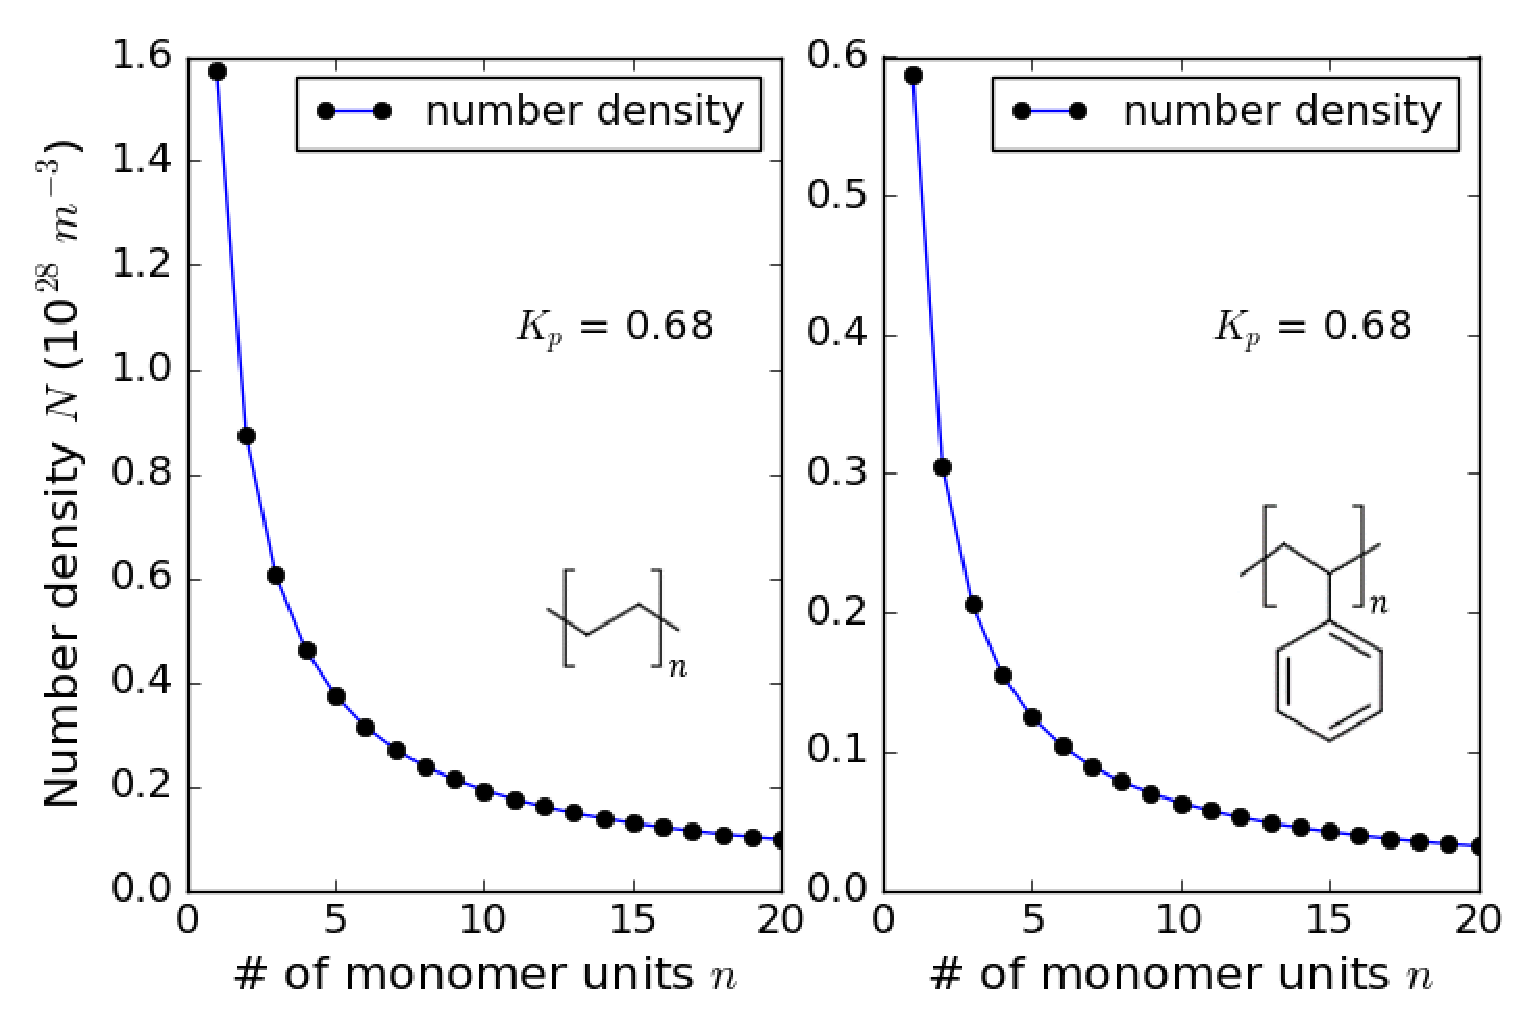
\includegraphics[width=0.75\textwidth]{Chapter-2/Figures/plot_numden.eps}
	\caption{Change of number density values for increasing degree of polymerization for the PE and PS prototype systems.} 
	\label{fig:nden_ex} 
\end{figure} 


Note that we can use this approach to compute another property of interest in organic materials research, \ie  the density $\rho$ of amorphous polymers in the bulk (\via\ $\rho = N \cdot N_A / M$ with the Avogadro number $N_A$ and molecular weight $M$). The density results for our prototype systems are presented in Fig.\ \ref{fig:den_ex}. 
% Discuss the variation of density (asymptotic behavior) with chain length using the same packing fraction for all oligomer length. 
The plots show that $\rho$ increases and ultimately convergences towards asymptotically constant values. This finite size effect due to the terminal groups is typically of limited magnitude. 
% Point out that calculation of density of 50 chain length polymer is a good representation of polymer limit.
The results of the oligomers with $n=50$ offer a good representation of the polymer limit and can thus be used as the default for determining $\rho$. The resulting densities are in very good agreement with experimentally known values \cite{Bicerano2002}. 
% Note that the Bicerano2002 paper reports the density values (gm/cm3) and not the number density values.
We can also use $\rho$ to work backwards and obtain the actual $K_p$ values. For PE and PS we obtain 0.64 and 0.66, respectively, \ie  using the average packing fraction of 0.68 happened to be a valid assumption in these particular cases.


\begin{figure}[htbp] 
	\centering
	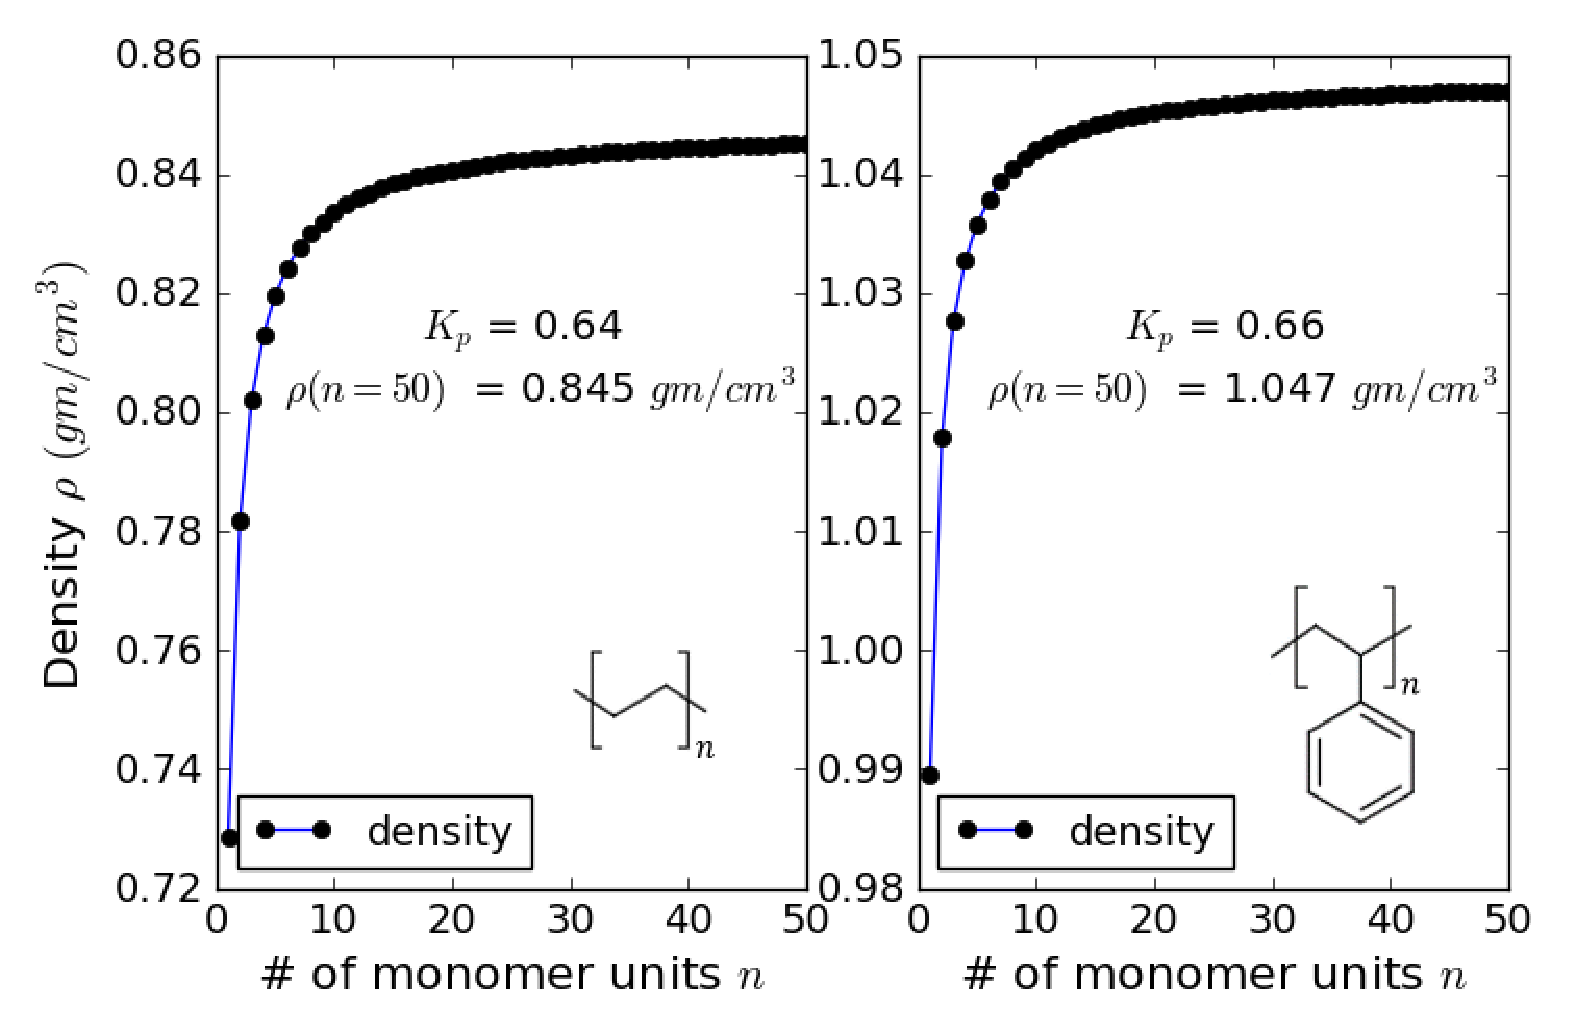
\includegraphics[width=0.75\textwidth]{Chapter-2/Figures/plot_den.eps}
	\caption{Change of density for increasing degree of polymerization for the PE and PS prototype systems. Note the characteristic asymptotic convergence to a constant value.}
	\label{fig:den_ex} 
\end{figure} 



\subsection{Packing Fractions}
\label{subsec:packingfractions_results}
% Explain that the packing fraction of targeted polymers is usually not known and therefore a prediction model is required
As $K_p$ is generally not known and the average value referenced in the literature \cite{askadski2003} is of limited utility, we have devised an SVR data model that correlates the polymer structure with the packing fraction as outlined in Sec.\ \ref{subsec:numberdensity} and \ref{subsec:compdetails}.
% Discuss the histogram of packing fractions of 84 polymers obtained from experimental density values and also on the range of the distribution
Fig.\ \ref{fig:Kp_hist} displays the range and distribution of $K_p$ values for the 84 polymers for which we found experimental results. 
%(either for $K_p$ or $\rho$)
This data -- ranging from 0.53 to 0.79 with an average value of 0.67 -- formed the basis for our data-derived $K_p$ prediction model. (Note that the average $K_p$ for our data set is nearly identical with the average $K_p=0.68$ cited in Ref. \cite{askadski2003}). 

% TODO: Do we have a plot of experimental vs ML K_p? potentially swap against Kp_hist
% Atif: Regarding the comparison of experimental and predicated Kp values, the issue is which graph to show. Should we present the correlation that use complete data for training or the correlation with 80-20 split for training and test respectively? I included a plot  for the latter (Kp_comparison.png and Kp_comparison.eps) in the folder 11/11_RI_prediction/pics/new_pics. I believe showing the histogram and including statistical data for the model would be less confusing.
\begin{figure}[htbp] 
	\centering
	\includegraphics[width=0.6\textwidth]{Chapter-2/Figures/Kp_hist.eps}
	\caption{Range and distribution of experimental packing fraction values for 84 polymers used in the creation of our data-derived prediction model.} 
	\label{fig:Kp_hist} 
\end{figure} 

% Results of SVR model
% Show the results of data modeling for the accurate prediction of packing fraction of polymers using SVR machine learning. Discuss the performance and the speed of the model.
The model gives an $R^2$ of 0.97 for the training and 0.87 for the test set. The performance drop for the latter is reasonable and acceptable given the small size of the available data set.
The computational demand for the $K_p$ prediction model is negligible and results for even large-scale compound libraries can be obtained in minutes on a single processor. 


\subsection{Refractive Indices}
\label{subsec:RI_results}
% Discuss resulting RI model that combines the results from polarizability and number density of these polymers and put in Lorentz-Lorenz equation to get RI values. 
Given the modeling protocols and resulting data for $\alpha$, $V_{vdW}$, $K_p$, and $N$, we use the Lorentz-Lorenz equation to make RI predictions.    
% Results of RI calculation of PE and PS prototype systems and comparison with experimental values; discuss the variation of RI values with the increasing chain length. 
Using the $\alpha$ and $N$ values obtained for our PE and PS prototype systems as shown in Figs.\ \ref{fig:pol_lin} and \ref{fig:nden_ex}, we calculate the RI values and their variation with the number of monomer units $n$ given in Fig.\ \ref{fig:RI_ex}. The RI increases for longer oligomers before reaching a plateau for $n=20$ to $30$. 


\begin{figure}[htbp] 
	\centering
	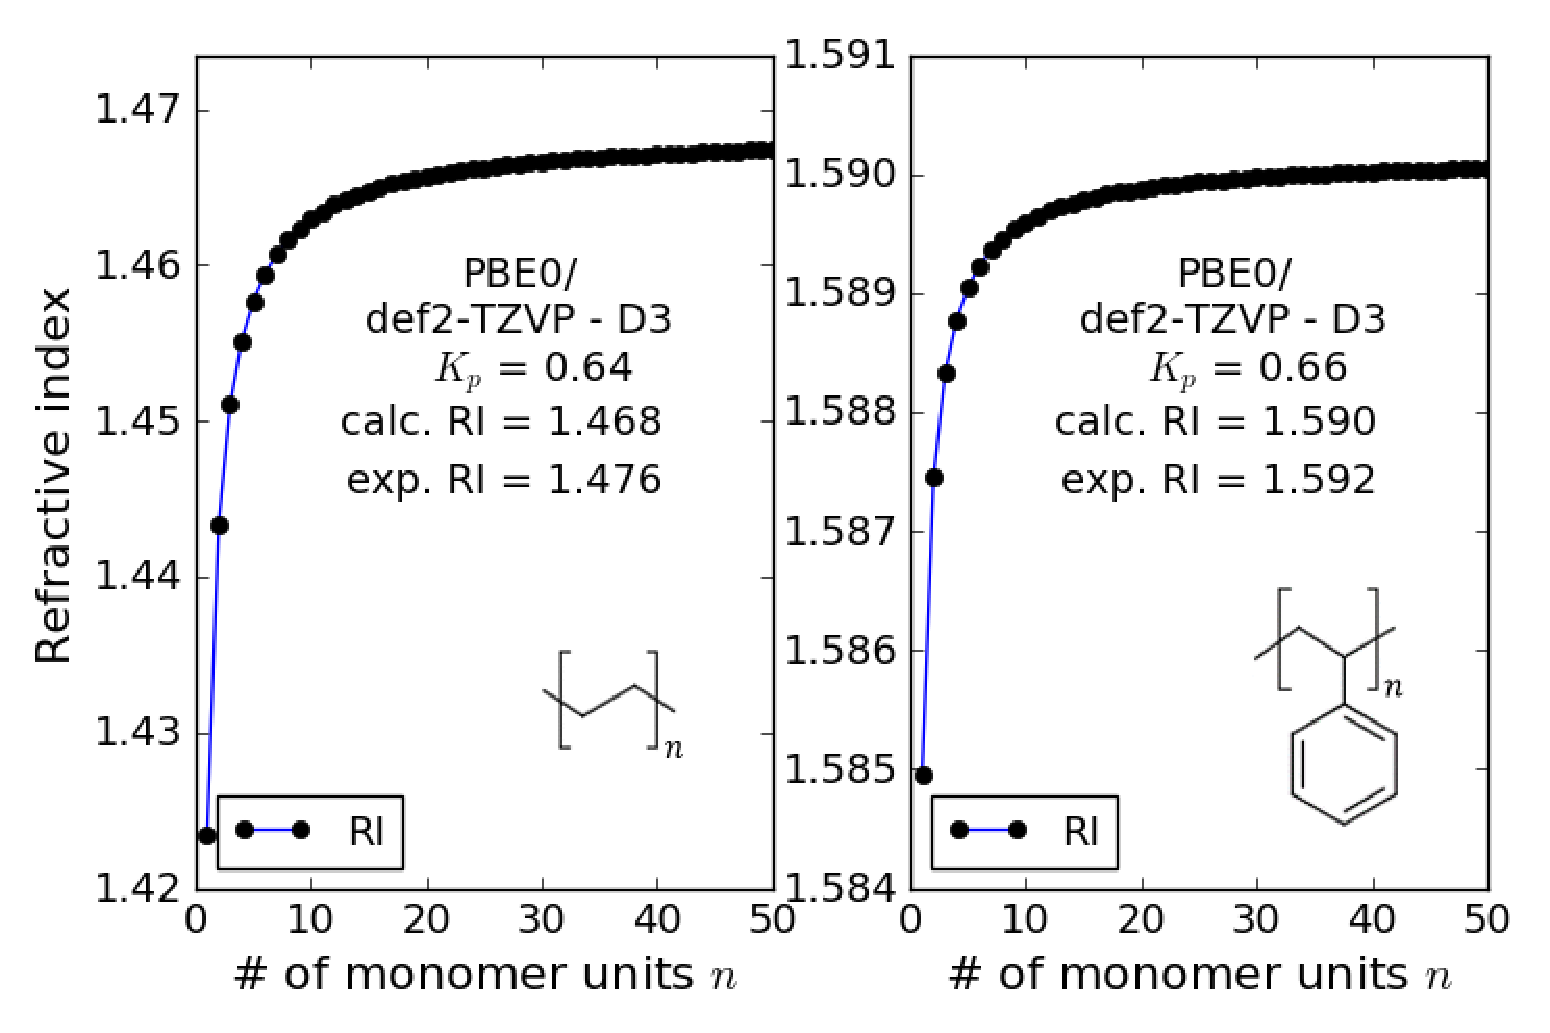
\includegraphics[width=0.75\textwidth]{Chapter-2/Figures/plot_RI.eps}
	\caption{Change of refractive index (RI) with increasing degree of polymerization for the PE and PS prototype systems. Note the characteristic asymptotic convergence to the constant value at the polymer limit, that is in excellent agreement with the experimental data.} 
	\label{fig:RI_ex} 
\end{figure}  


% Comparison with experimental results
Our modeling protocol predicts the RI values for PE and PS to be 1.468 and 1.590, respectively, which is in outstanding agreement with the experimental RI values of 1.476 and 1.592, respectively \cite{Bicerano2002}.
% Now that we have developed a model for the prediction of RI values of polymers, we validate it by testing against the experimental RI values of 112 polymers. 
We further validate our modeling protocol by predicting the RI values of 112 polymers for which we could find experimental data for comparison (see Fig.\ \ref{fig:validation}). 



% \begin{figure}[htbp] 
\begin{figure}[hbpt] 
	\centering
	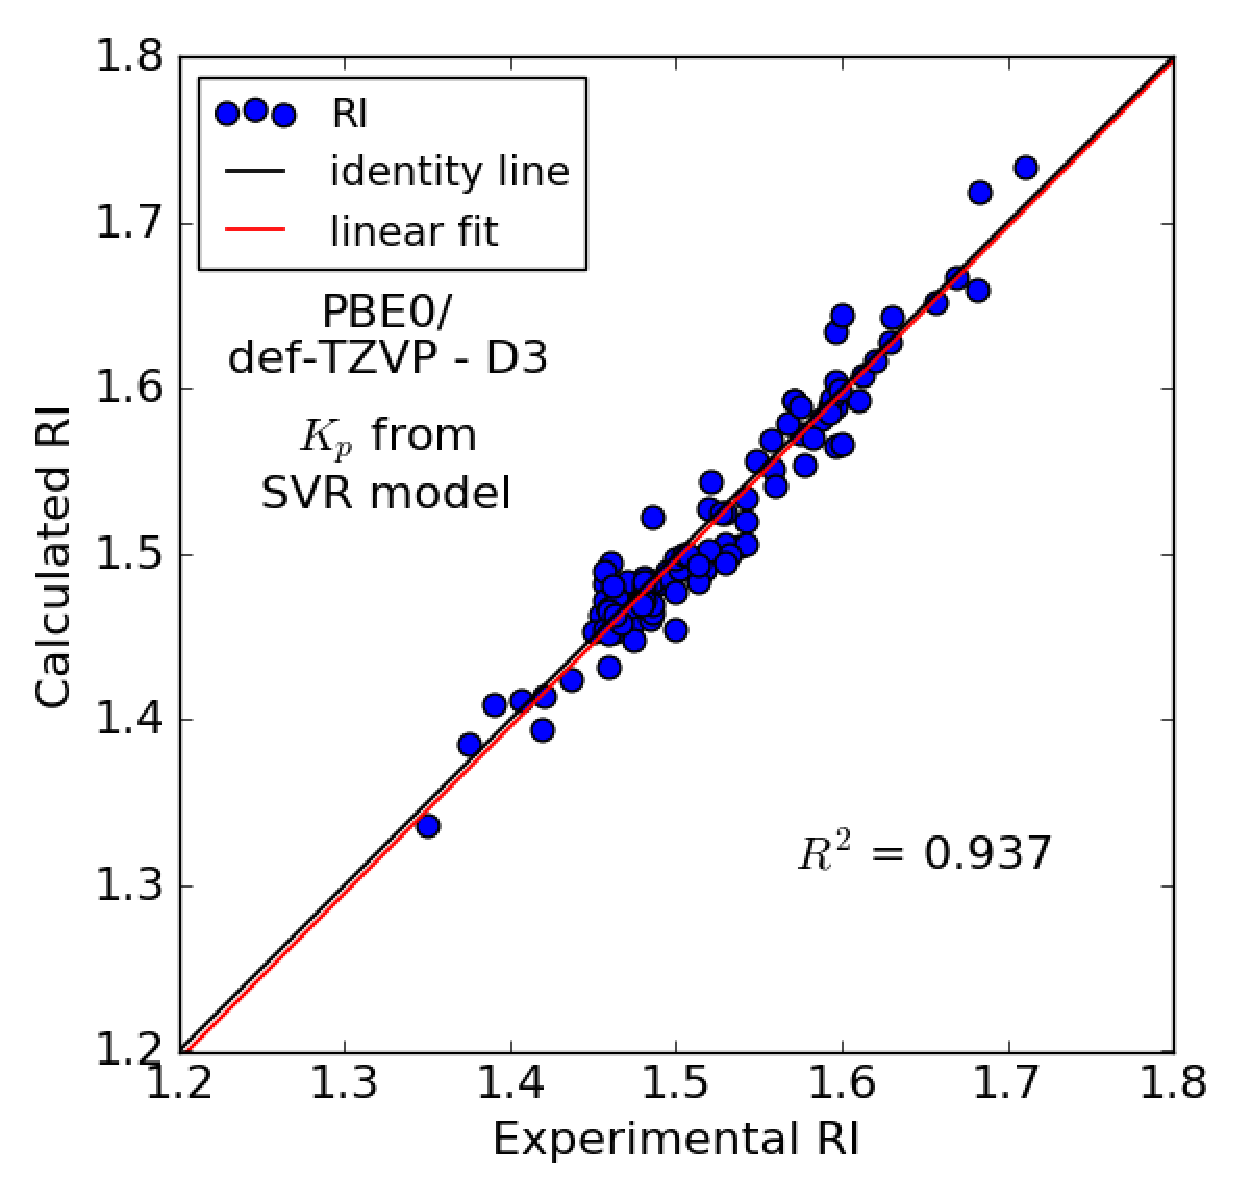
\includegraphics[width=0.6\textwidth]{Chapter-2/Figures/PBE0_Kp_ML.eps}
	\caption{Validation of the proposed RI prediction model (based on the data-derived model for the packing fraction) through comparison with 112 experimental data points.	
	} 
	\label{fig:validation} 
\end{figure} 


% Discuss the performance of the model. 
The $R^2$ of 0.94 shows that the model is in very good agreement with the experimental RI values. The benchmark comparison gives a mean absolute deviation (MAD) of 0.010 (0.9\%), a root mean square deviation (RMSD) of 0.018 (0.1\%), and a maximum deviation (MaxD) of 0.045 or 3.0\%, respectively, \ie  our modeling protocol is quite accurate and affords at least semi-quantitative predictions (in particular since typically only two decimals in the RI values are considered as significant). The average deviation (AD) is very small with +0.004 (+0.3\%), \ie  our model is not significantly biased towards systematic over- or under-predictions. A result of particular importance for studies that focus on candidate rankings rather than quantitative predictions for individual candidates is that the trends in the data are generally well captured. We stress that the experimental RI data is independent of the data used for the creation of the SVR model for $N$, \ie  the SVR model was not biased towards providing good RI results.

% TODO: add to Supplementary Material with only 3 decimal places 
% more analysis
% R_squared	0.936796097
% RMSD	0.017886417
% Mean_error	0.003894643
% Average_error	0.003894643
% Median_error	0.0048
% STD_error	0.017457253
% Variance_error	0.000304756
% Max_error	0.045
% Min_error	-0.0437
% SPR_error	0.0887
% Mean_perc_error	0.916655011
% Confidence_interval_95_l	0.000611248
% Confidence_interval_95_u	0.007178038
% t_test	0.425647902
% p_value	0.670777354

For comparison, using the average packing fraction value of 0.68 -- as is oftentimes cited in related work -- instead of our SVR model leads to the results shown in Fig.\ \ref{fig:validation_const_Kp}. This model is considerably worse, as can be seen from the $R^2$ of 0.78, MAD of 0.019 (1.9\%), RMSD of 0.026 (0.3\%), MaxD of 0.139 and 6.9\%, and AD of $-$0.009 ($-$0.6\%).

\begin{figure}[htbp] 
	\centering
	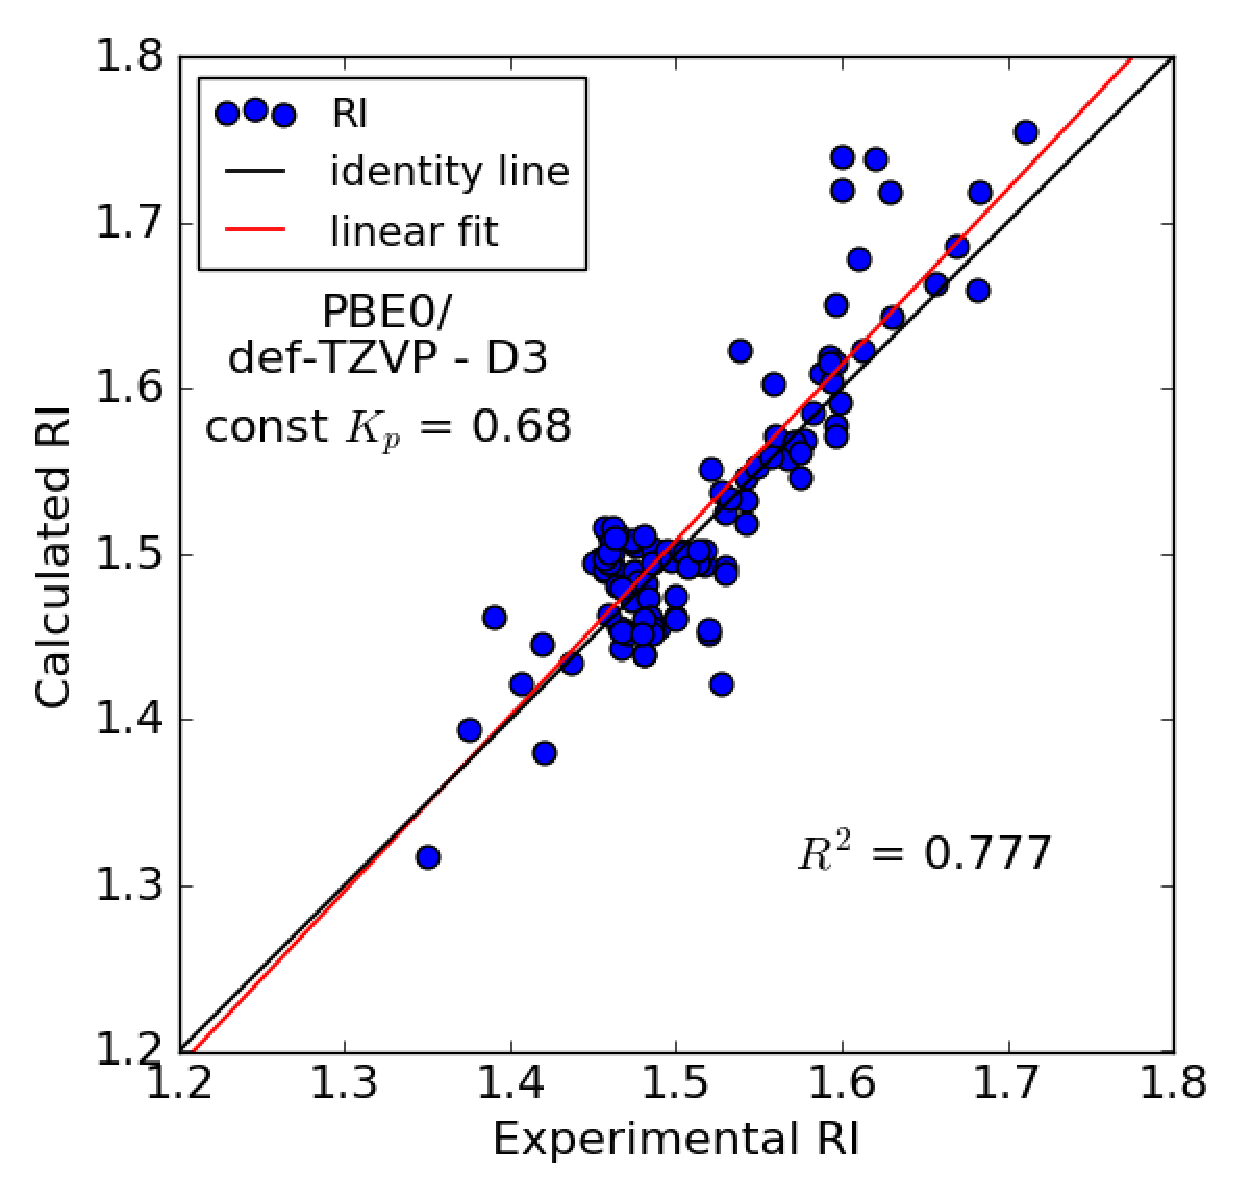
\includegraphics[width=0.6\textwidth]{Chapter-2/Figures/PBE0_Kp_068.eps}
	\caption{Validation of an RI prediction model based on a constant average packing fraction.} 
	\label{fig:validation_const_Kp} 
\end{figure} 

% \textcolor{red}{
The before-mentioned pioneering work by Ramprasad \etal\ offers another instructive reference point. It creates a machine learning prediction model for the dielectric constant ($\epsilon_r = {n_r}^2$) of organic and organometallic compounds that is based on training data from plane-wave DFT for crystalline systems \cite{Huan2016,Sharma2014}. Ramprasad’s database includes 7 experimental data points that can be used for the validation of the underlying DFT model \cite{Mannodi-Kanakkithodi2016}. The DFT predictions show a correlation of only $R^2 = 0.78$ with respect to the experimental data. This suggests that the use of DFT crystal structures may be the cause of some loss in predictive performance, which can propagate into the derived machine learning models. This observation underscores the importance of accurately accounting for the amorphous bulk structure, which our approach achieves. 
% }

% \textcolor{red}{
It is worth stressing that while our discussion focused on non-conjugate polymer examples, our computational protocol can also be employed on conjugate systems provided the extensive regime is considered in the extrapolation schemes. The SVR prediction model for $K_p$ was trained on typical organic polymers and may start to fail for unusual or extreme cases that were not represented in the training set. In such a situation it would be advisable to retrain the model with more targeted training data. 
% }


\subsection{Interplay between Polarizability and Number Density}
\label{subsec:interplay_results}
% Analyze interplay of alpha and N because they are the input slots of the model; do this for our experimental data set
As the Lorentz-Lorenz equation relies on $\alpha$ and $N$ as input parameters, we analyze their interplay for the 112 polymers in our validation and benchmark data set.
% Plot relationship between the polarizability and number density using the values of 112 polymers. 
% Atif: The $\alpha$ and $N$ shown in the relationship plot represent the values for a polymer chain with 50 monomer units.
Fig.\ \ref{fig:relationship} shows the calculated $\alpha$ and $N$ values as well as the contour lines for the resulting RI values in this parameter space. 

\begin{figure}[htbp] 
	\centering
	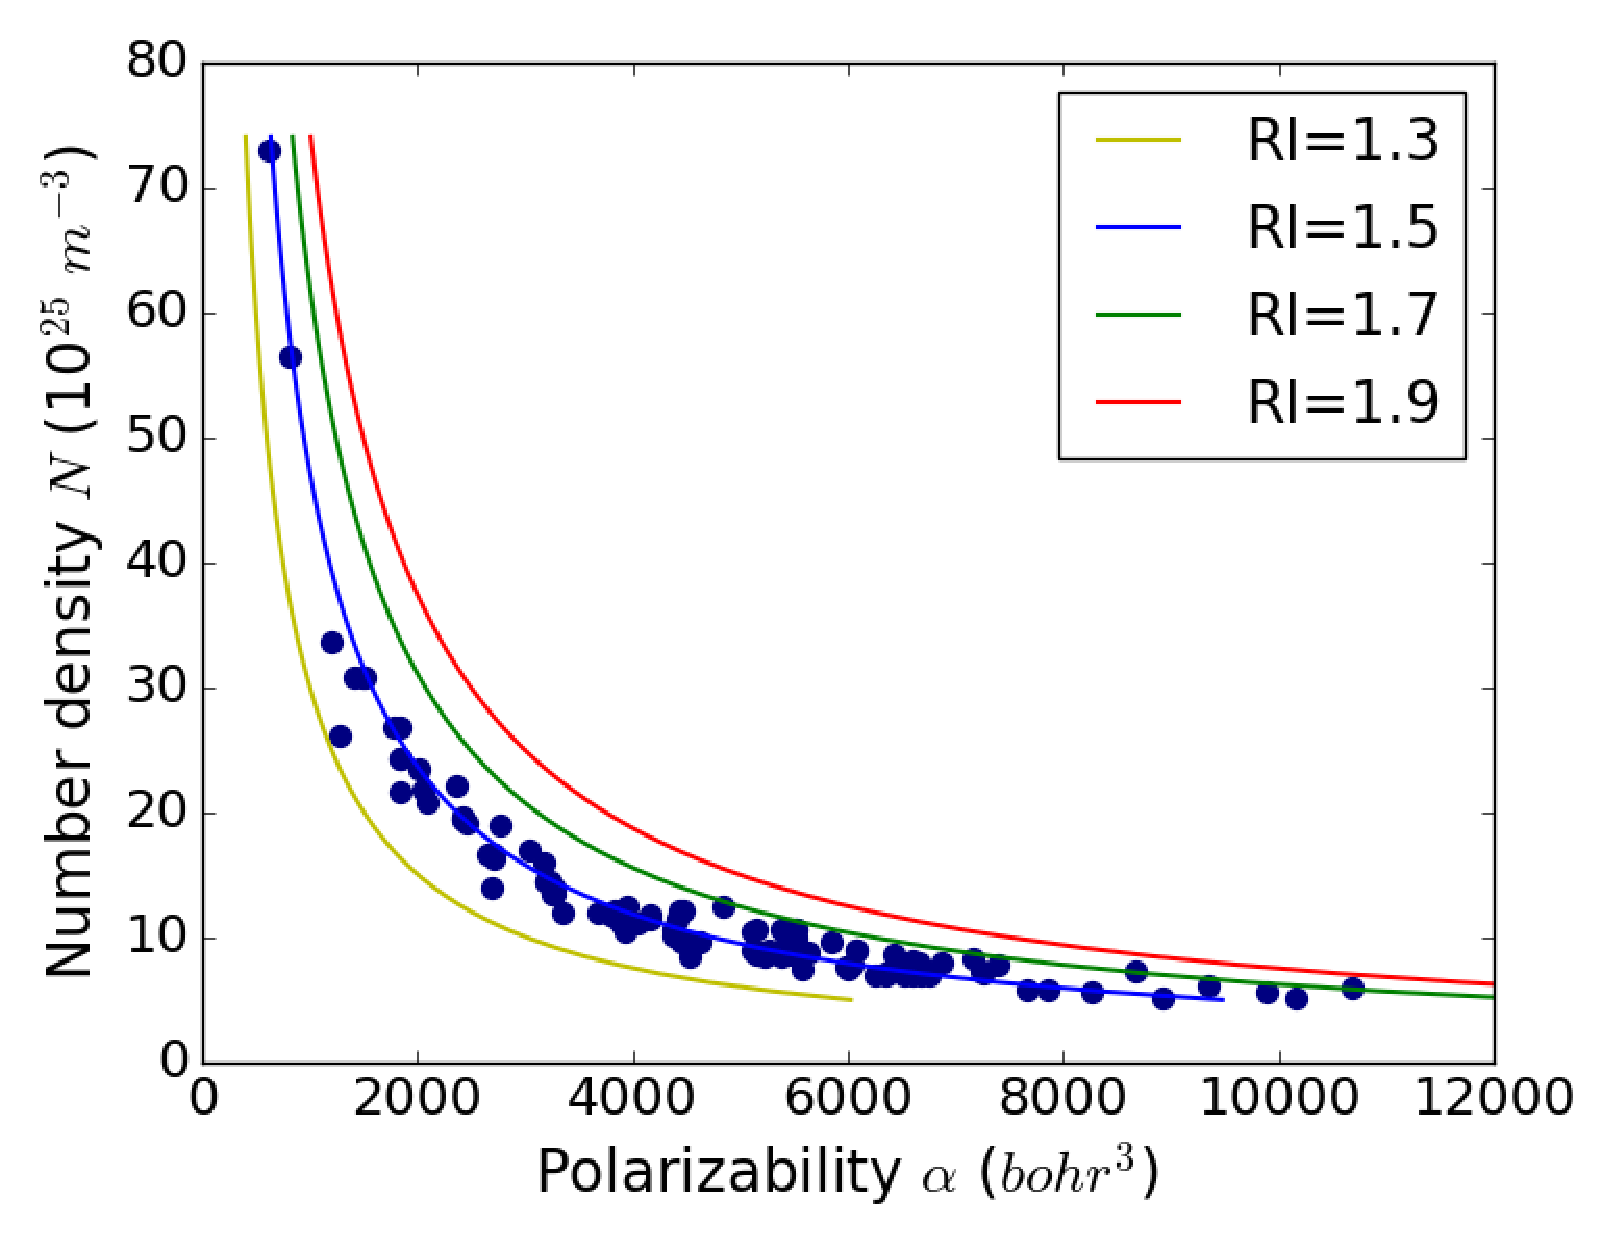
\includegraphics[width=0.6\textwidth]{Chapter-2/Figures/Den_vs_pol_contour.eps}
	\caption{Parameter space of polarizability $\alpha$ and number density $N$ as well as resulting RI value domains with examples from our validation and benchmark data.} 
	\label{fig:relationship} 
\end{figure} 

% Discuss the regions of high RI values and potential pathways of moving towards these regions. Give future directions for the quest of high-RI polymers
To achieve high RI values, a candidate compound must feature both large number density and polarizability values (as is also apparent from the structure of the Lorentz-Lorenz equation). Optimizing both properties simultaneously is a challenging task as extensivity couples $\alpha$ and $N$, \ie  the longer a polymer, the larger $\alpha$ (as $\alpha$ increases with the number of contributing monomer units), but the smaller $N$ (as fewer molecules fit into a given volume element). A design strategy that can be derived from this notion is to incorporate highly polarizable moieties that have a limited effect on the number density. The data set at hand is tilted towards a larger spread in $\alpha$ while $N$ is more clustered. It is worth noting that the RI regions in the $\alpha$ \textit{vs} $N$ parameter space are relatively narrow and most compounds in the data set group around the contour line for RI=1.5. The high-RI examples primarily stand out for large polarizability values rather than large number densities, which supports the before-mentioned design strategy.

% suggests, indicates

% this is basically a repetition of the abstract in rephrased, perhaps more concrete form
\section{Conclusions}
\label{sec:conclusions} 
We have successfully developed a modeling protocol for the accurate prediction of the RI values of organic polymeric materials and validated it against the experimentally known RI values of 112 compounds. The current work is an example for the benefits of fusing physical and data models, with the former providing the general structure of the approach (\ie  the Lorentz-Lorenz equation) and a significant part of the required input parameters (\ie  polarizabilities from \firstprinciples\ quantum chemistry and van der Waals volumes from Slonimskii's method), while the latter provides rapid access to input data that is otherwise not readily available (\ie an SVR model for the packing fraction and an extrapolation scheme for molecular results towards the polymer limit). A subset of our RI protocol can also be used to predict the density of amorphous polymers. Our work is furthermore an example for the great promise of applying machine learning and modern data science in chemical research. In later chapters, we will utilize this new RI protocol to conduct virtual high-throughput screening studies on large-scale candidate libraries with the goal of accelerating the discovery of novel organic materials with unprecedented RI values.
